%ファイル分割をいい感じにする
\documentclass[_main]{subfiles}

\begin{document}
\chapter{章タイトル}
\section{節タイトル}

\begin{figure}
  \centering
  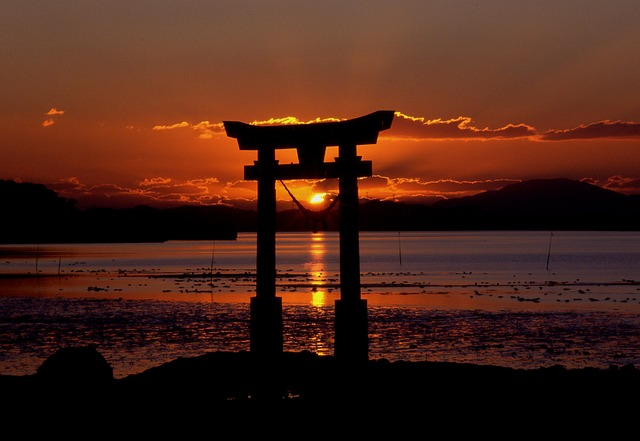
\includegraphics[height=6cm]{sample.jpg}
  \caption{神社}
  \label{shrine}
\end{figure}

表\ref{charas}は、あるアニメ群の主要な登場人物数を示すものです。

\begin{table}[htbp]
\begin{center}
\caption{アニメの登場人物数}
\begin{tabular}{ll}
タイトル & 主要登場人物数\\ \hline
K & 4\\
Y & 7\\
G & 9くらい\\
S & 100くらい\\ \hline
\end{tabular}
\label{charas}
\end{center}
\end{table}


\end{document}
